%% Template for MLP Coursework 3

%% Based on  LaTeX template for ICML 2017 - example_paper.tex at 
%%  https://2017.icml.cc/Conferences/2017/StyleAuthorInstructions

\documentclass{article}
\usepackage[T1]{fontenc}
\usepackage{amssymb,amsmath}
\usepackage{txfonts}
\usepackage{microtype}
\usepackage{xspace}
\xspaceaddexceptions{\%}

% Lists with less spacoing between items
\usepackage{paralist}

% For figures
\usepackage{graphicx}
\usepackage{subfig} 

% For citations
\usepackage{natbib}

% For algorithms
\usepackage{algorithm}
\usepackage{algorithmic}

% the hyperref package is used to produce hyperlinks in the
% resulting PDF.  If this breaks your system, please commend out the
% following usepackage line and replace \usepackage{mlp2017} with
% \usepackage[nohyperref]{mlp2017} below.
\usepackage[hyphens]{url}
\urlstyle{same}
\usepackage{hyperref}

% Packages hyperref and algorithmic misbehave sometimes.  We can fix
% this with the following command.
\newcommand{\theHalgorithm}{\arabic{algorithm}}


% Set up MLP coursework style (based on ICML style)
\usepackage{mlp2018}
\mlptitlerunning{MLP Coursework 3 -- Interim Report (\groupNumber)}
\bibliographystyle{icml2017}


\DeclareMathOperator{\softmax}{softmax}
\DeclareMathOperator{\sigmoid}{sigmoid}
\DeclareMathOperator{\sgn}{sgn}
\DeclareMathOperator{\relu}{relu}
\DeclareMathOperator{\lrelu}{lrelu}
\DeclareMathOperator{\elu}{elu}
\DeclareMathOperator{\selu}{selu}
\DeclareMathOperator{\maxout}{maxout}






\usepackage[utf8]{inputenc}
\pagenumbering{arabic}

%% You probably do not need to change anything above this comment
%Reference Numbers of Images Used:
%58c593bcb98386e7fd42a1d34e291db93477624b164e83ab2afa3caa90d1d921
%00ae65c1c6631ae6f2be1a449902976e6eb8483bf6b0740d00530220832c6d3e
%0bda515e370294ed94efd36bd53782288acacb040c171df2ed97fd691fc9d8fe

%% REPLACE this with your project title, group ID and list of student numbers for the group
\def\projectTitle{Segmentation of Nuclei in Biomedical Imagery}
\def\groupNumber{G108}
\def\studentNumbers{s1515679, s1553593}

\begin{document} 

\twocolumn[
\mlptitle{\projectTitle: Final Report}

\centerline{\groupNumber\ (\studentNumbers)}

\vskip 7mm
]

\begin{abstract} 
\iffalse
The abstract should be a few sentences (100--200 words) long,  providing a concise summary of the contents of your report including the key research question(s) addressed, the methods explored, the data used, and the findings of the experiments. \cite{Ronneberger2015UNetCN}
\fi 

In this report, we will investigate the use of segmentation in biomedical images, making predictions on a per-pixel basis to create masks for the test data. The report explores modern techniques for semantic segmentation  such as Fully Convolutional Networks and U-Net. Our experiments are conducted over hundreds of microscopic images of cells in an attempt to identify, detect and extract nuclei from these images. The generated masks could have powerful applications in the biomedical industry - automating the analysis of microscopic images will accelerate the discovery of cures, assisting experts in the field with their research. Given that the dataset is fairly small, we investigate the use of various models and data augmentation techniques and evaluate the effect of an expanded dataset size.
\end{abstract} 

\section{Introduction}
\label{sec:intro}
For the 2018 Data Science Bowl, Booz Allen Hamilton created a Kaggle competition to task people to find the nuclei in divergent images to advance medical discovery \cite{KaggleComp}, with only around 650 examples. In this report we will analyse a variety of different Convolutional Neural Networks (CNNs) and data augmentation techniques, to try and produce automatic segmentation of microscopic nuclei images with this very small dataset.

To find these nuclei we have framed this task as a semantic segmentation \cite{semsegslides} problem. The goal is to understand the parts of an image at pixel level, we want to know what object(s) are in the image and where in the image the object(s) are. In this report, our goal is to classify each pixel into one of two classes; nuclei and not nuclei. In doing this, we achieve fine-grained inference and a classification for every pixel in the image (a dense prediction). Semantic segmentation itself is a structured prediction task, which is much more complex than a simple classification task. This is because we attempt to predict objects containing some internal structure rather than a simple binary classification or regression \cite{structuredpredthesis}.

In this report, we implemented our models in PyTorch \citep{pytorch} and used preprocessing and data augmentation techniques in Python to answer the following research questions:
\begin{samepage}
\begin{enumerate}
    \item \textbf{Does a state-of-the-art U-Net model provide improvements over a Fully Convolutional Network in the biomedical domain, after extensive hyperparameter tuning?}
    Fully Convolutional Networks (FCNs) were designed to solve semantic segmentation problems. An adaptation of FCN was designed, called U-Net, targeting biomedical imagery. We will investigate how significant the improvements (if any) are, using U-Net.  
    \item \textbf{How does data augmentation improve both U-Net and a Fully Convolutional Network with a very small dataset?}
    The dataset that we are using contains only around 650 images, this is a very small amount of data for a semantic segmentation task. We will attempt to tackle this small data problem and analyse the effect of data augmentation on our models. Given that U-Net is efficient and lightweight, it should work well on small datasets. Therefore we believe it will be interesting to investigate the effect of augmentation on IoU accuracy, compared to FCNs.
\end{enumerate}
\end{samepage}
 
%In this report, we intend to investigate and optimise different Convolutional Neural Networks (CNNs) and image processing approaches to try and find which performs best at identifying nuclei in images. 
% In this report we will be analysing and tackling the different issues with the Kaggle competition to try and tackle the small data problem that was present in the competition.
We will begin by analysing our classification accuracy with completely black, white and random pixel classification masks as a baseline. We will then look at FCNs and U-Nets to see how each of these handles the semantic segmentation problem. We chose a U-Net model because we only had 500 images available as training data and in \cite{MicrosoftUnetSmallData}, a U-Net was implemented for the semantic segmentation of satellite images with less than 100 annotated satellite images. We chose FCNs because U-Nets are a type of FCN that were developed specifically for biomedical image segmentation \cite{Ronneberger2015UNetCN} and FCNs have been found to be particularly useful in other semantic segmentation tasks \cite{Long2015FullyCN}.

FCNs and U-Nets are based on CNN architectures. There has been a boom in the computer vision space due to the advances in technology that have reduced the training time of these CNNs, advanced cluster computing, and created more powerful GPUs that allow parallel computing. CNNs have proved to be very useful in this problem space \citep{historyAlexNet} because of their similarity with the human vision system.

The output of this task has very important applications, by enabling automatic segmentation of nuclei in images, we can assist researchers and medical experts with manual annotation tasks. In doing so, we reduce the amount of time these experts spend on this process, enabling them to commit more time to more important research. Hopefully this automatic annotation will help reduce human error, reduce cost, and speed up the process of finding cures.

One of our original objectives was to include a Mask-RCNN architecture in our experimentations \cite{MaskRCNN}. Mask-RCNN is a model that attempts to solve instance segmentation in computer vision tasks. Instead of just classifying as nuclei or not, instance segmentation classifies nuclei individually e.g. nucleus1, nucleus2 etc. We believed this would be useful because it would allow us to isolate separate nuclei and reduce the problem of two nuclei forming one merged shape (as seen in Figure \ref{fig:prediction}). By introducing gaps between neighbouring nuclei we would hopefully be able to increase our IoU scores. The basis for Mask-RCNN stems from Feature Pyramid Networks (FPNs) \cite{Lin2017FeaturePN}. This is the reason for most of the problems we encountered with this model; FPNs are generally very memory intensive and computationally slow, and more importantly they require much more data than the other models we are using. Therefore we believe that our dataset was simply too small to train the model to a level that was useful for this task. However, in the Kaggle competition, some teams were able to use these networks and get great results. This was because they were able to access additional biomedical data, and with a lot of reformatting and processing, helped improve the small data problem that we had.

\section{Data set and task} 

The dataset that we will be using was provided by Booz Allen Hamilton for the Kaggle competition, ``Data Science Bowl 2018''. It consists of 667 RGB images of nuclei and the corresponding ground truth binary masks of each nucleus.
%which we decided to split into a train:validation:test split of 75:15:10 which resulted in 500 training, 100 validation, and 67 test images. 
% Each image has a set of different masks for each nucleus in each image. For example Figure \ref{fig:TrainImage}, shows how a training image looks like and Figure \ref{Fig:Masks} shows the corresponding masks, showing the nuclei. However, for our evaluation metric we need to have the masks as 1 image and so we combine the masks in the image resulting in an image with all the masks as seen in Figure \ref{fig:MasksCombined}.
%However for the evaluation of our models we will combine these mask images into a single image?

For each raw microscopic image, there is a set of masks for each nucleus in the image e.g. for a raw image containing 5 nuclei there would be 5 corresponding mask images. For our training data, we iterated over each mask and combined them into one image, which enabled us to have training labels that would be comparable with our predicted output segmentation masks. An example of the data that we are using for training purposes can be seen in Figure \ref{fig:example_images}.

% \begin{figure}[ht]
% \vskip 5mm
% \begin{center}
% \centerline{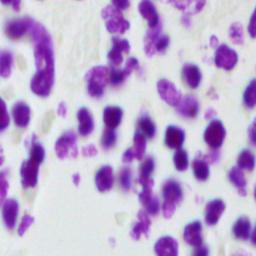
\includegraphics[scale=0.5]{mlp-cw3-template/Figures/raw_nuclei.jpg}}
% \caption{A sample raw microscopic training image.}
% \label{fig:TrainImage}
% \end{center}
% \vskip -5mm
% \end{figure} 


\begin{figure}[ht]
\vskip 3mm
\begin{tabular}{ll}
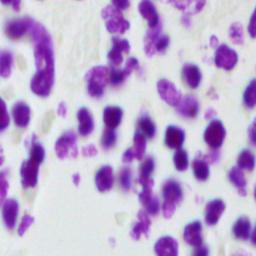
\includegraphics[scale=0.40]{mlp-cw3-template/Figures/raw_nuclei.jpg}
&
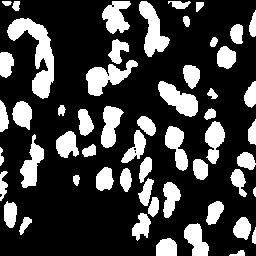
\includegraphics[scale=0.56]{mlp-cw3-template/Figures/ground_truth_nuclei.jpg}
\end{tabular}
\caption{An example of a raw microscopic image, in the data set, and its corresponding ground truth binary mask (label), after the combination process.}
\label{fig:example_images}
\vskip 1mm
\end{figure}

% \begin{figure}[ht]
% \vskip 5mm
% \begin{center}
% \centerline{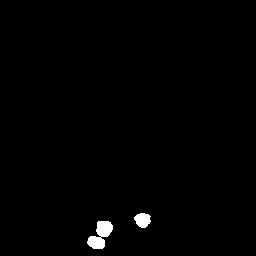
\includegraphics[scale=0.5]{mlp-cw3-template/Figures/2MasksCombined.png}}
% \caption{Masks from Figure \ref{Fig:Masks} combined}
% \label{fig:MasksCombined}
% \end{center}
% \vskip -5mm
% \end{figure} 

The images consist of different magnifications, dimensions, and fluorescence. Typically, the images consist of 256x256 pixels however sometimes the dimensions don't fit this pattern, as in the case of Figure \ref{fig:DifferingTrains}(b), and the pixel density can also go as far as 1040x1388. To combat this and provide consistency of our images we resized all of our images and masks to the typical 256x256 format. To reduce the size of the rectangular images, the smaller of the image edges were matched to output size (256x256), therefore keeping the aspect ratio the same. Additionally, the cells in the same image may be of a different type and have a different luminosity. Figure \ref{fig:DifferingTrains}, illustrates this. As we can see, the images and cells can vary vastly. This high variance in a small dataset introduces additional problems, further substantiating our need for data augmentation - increasing the amount of training data and reducing the variance.

\begin{figure}[htbp]
    \vskip 5mm
    \centering
    \subfloat[Image with Multiple Cell Types]{{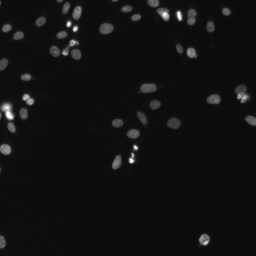
\includegraphics[scale=0.4]{mlp-cw3-template/Figures/VaryingImg.png}}}%
    \qquad
    \subfloat[Image taken with added fluorescence]{{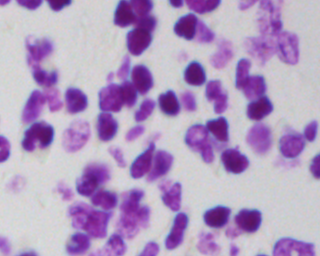
\includegraphics[scale=0.33]{mlp-cw3-template/Figures/PurpleImg.png} }}%
    \caption{Further Sample Training Images Illustrating Cell and Image Variation}%
    \label{fig:DifferingTrains}%
    \vskip 1mm
\end{figure}

We decided to hold-out 10\% of the images for our testing set, the test set was selected so that we had a similar variance in images as the training set, the test set would then hold a true representation of the dataset. We then used 6-fold cross-validation on the remaining 600 images for training and validation. We decided to use a cross-validation approach because it will help avoid overfitting, which could be a problem, due to our dataset. Also, because the cell images vary quite widely we wanted to ensure that the splitting of the images was as fair as possible, reducing the bias as much as possible for the training process.

The accuracy of our models will be evaluated using an IoU (Intersect over Union) score (also called the Jaccard Index) \cite{Tan2005IntroductionTD}. This evaluation metric is very common in the semantic segmentation domain, but slightly different to the evaluation metric used in the Kaggle challenge. Therefore, we can't directly compare our models' performance to the winning Kaggle solutions. The Jaccard Index can have a value between 0 and 1, the equation can be seen below:

% \[ J(x,y) = - \sum_{i=1}^{d_x} x_i \log(y_i) + (1 - x_i)\log(1-y_i)\]

\[ J(x,y) = \dfrac{|A \cap B|}{|A \cup B|} = \dfrac{|A \cap B|}{|A|+|B|-|A \cap B|}\]
where A is the ground truth binary mask for the nuclei, annotated by a human with knowledge in the biomedical field and B is the  predicted binary masks for each raw microsopic image. IoU measures the amount of overlap between these two masks. To explain this overlap further, see Figure \ref{fig:iou}.

\begin{figure}[ht]
\vskip 5mm
\begin{center}
\centerline{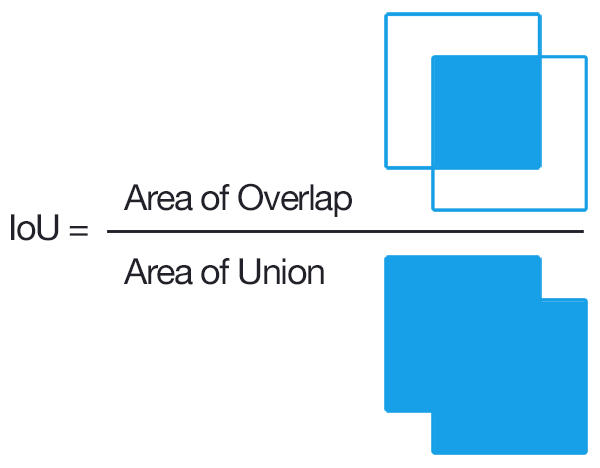
\includegraphics[scale=0.19]{mlp-cw3-template/Figures/iou.png}}
\caption{A simplified version, showing the calculation for the IoU evaluation metric.}
\label{fig:iou}
\end{center}
\vskip -5mm
\end{figure} 

% By experimenting with the FCN and U-Net models, we hope to optimise and compare the performance of both of these models. After this point, we will attempt to apply various pre-processing to the images and see how both of the models improve when provided with more data.

\section{Methodology}

\iffalse
\begin{algorithm}[ht]
\begin{algorithmic}
   \STATE {\bfseries Input:} data $x_i$, size $m$
   \REPEAT
   \STATE Initialize $noChange = true$.
   \FOR{$i=1$ {\bfseries to} $m-1$}
   \IF{$x_i > x_{i+1}$} 
   \STATE Swap $x_i$ and $x_{i+1}$
   \STATE $noChange = false$
   \ENDIF
   \ENDFOR
   \UNTIL{$noChange$ is $true$}
\end{algorithmic}
  \caption{Bubble Sort}
  \label{alg:example}
\end{algorithm}
\fi

\subsection{Baseline}
\label{sec:baseline}
For our baseline, we decided to first look at the IoU accuracy if our model was to predict; 
all pixels as not nuclei, all pixels as nuclei and a random scattering of nuclei, based on the prior probabilities. The prior probabilities are the number of background pixels and number of nuclei pixels (in the ground truth labels), divided by all the pixels in the dataset. In this case, our priors are the following: $P(Background) = 0.868$ and $P(Nucleus) = 0.132$.

When the model predicts no nuclei we get a score of 0: $|A \cap B|$ $=$ 0 because none of the nuclei were correctly predicted. When the model predicts all the pixels as nuclei we get a score of 0.1318 which is the percentage of the images that consist of nuclei. We know this is the case because the IoU score would be as follows, where $|A|$ is the prior of the nuclei:
\[ J(x,y) = \dfrac{|A \cap B|}{|A \cup B|} = \dfrac{|A \cap B|}{|A|+|B|-|A \cap B|}\]
\[ = \dfrac{0.1318}{0.1318+1-0.1318} = 0.1318\]

If we predict the model to randomly be 13.18\% nuclei then we get a score of 0.0588, which is to be expected because most of our random nuclei predictions would miss where an actual nuclei was and so $|A \cap B|$ would perform poorly as in the all-black model. In fact, if we randomly set the nuclei then we typically got a score between 0 and 0.1318, the more all-white the closer it was to 0.1318. Therefore from our baseline we can tell that any score over 0.1318 is a model that is not randomly assigning values. These results can be summarised in Table \ref{tab:random_baseline}.

\begin{table}[htbp]
\vskip 3mm
\begin{center}
\begin{small}
\begin{sc}
\begin{tabular}{lcccr}
\hline
\abovespace\belowspace
Prediction technique & IoU Accuracy \\
\hline
\abovespace
All pixels are not nuclei & 0.0000 \\
All pixels are nuclei & 0.1318 \\
50\% are nuclei & 0.1079 \\
\belowspace
13.8\% are nuclei & 0.0588 \\
\hline
\end{tabular}
\end{sc}
\end{small}
\caption{IoU accuracies for baseline predictions.}
\label{tab:random_baseline}
\end{center}
\vskip -3mm
\end{table}

\subsection{Small Data Problem}
%13.2\% are positive - weighted cross entropy for imbalanced dataset. 
In \cite{WTDwSmallData} the following were quoted as problems with small data:
\begin{itemize}
    \item Overfitting becomes much harder to avoid.
    \item You don’t only overfit to your training data, but sometimes you overfit to your validation set as well.
    \item Outliers become much more dangerous.
    \item Noise in general becomes a real issue, be it in your target variable or in some of the features.
\end{itemize}
Therefore, we had to take into account the fact that these issues may be a problem and try to solve them as best as possible. In \cite{SmallDataCurse}, several approaches to help break the curse of small data were acknowledged. 

According to \cite{SmallDataCurse}, changing the loss function helps with classification with unbalanced data by adding weights to the losses to even out the bias. In Section \ref{sec:baseline} we identified that only 13.18\% of the images contains a nucleus, therefore we applied weights in the ratio of 13.18:86.82 (which equals 1:6.615) to the Cross-Entropy loss function calculation to target the data imbalance. We also tried using the Lovász-Softmax loss function \cite{berman2018lovasz} which was developed specifically to optimise IoU for neural networks.

We also tried inflating our dataset by applying preprocessing techniques to create new images for our dataset. How this was done is outlined in Section \ref{sec:ImgPreProcess}.

Lastly, to evaluate any overfitting of the validation set, we held out 10\% of our data for our test set which we will only evaluate our model on, at the very end.  

\subsection{Convolutional Neural Network}
\label{sec:CNN}
A convolutional neural network is a type of supervised artificial neural network that is very often used for image processing. Specifically, CNNs allow images to be processed on a per-pixel basis which has proved to work very well in practice \cite{Alom2018TheHB}. It is supervised because the network is trained using both input images (raw biomedical imagery) and labels (ground truth binary masks).

A CNN is an architecture that is often used in simple classification tasks, where a single class label would be given for each image e.g. cat or dog. However, they are also widely used for image segmentation tasks. It is built from an input layer, hidden layers in between and an output layer. The hidden layer usually consists of multiple types of layer such as convolutional, max pooling, fully-connected and up-sampling layers \cite{CNNExplained} provides a detailed explanation of these layers). The network will learn the filters that would otherwise have to be designed by a person, removing the need for feature engineering. This independence from human interaction and an increase in efficiency, makes CNNs very advantageous.

% For our baseline, we will use a CNN. Typically CNNs are used for classification of images. However for the nature of this task we will be using them for image segmentation. Therefore, for our baseline we will be utilizing CNNs as described in \cite{pinheiro2014} to classify images on a per-pixel basis. This per-pixel CNN classifier is also known as a Fully Convolutional Network \cite{Long2015FullyCN}. In an FCN, there is no fully connected layer and instead the output is the same size as the input. An example of the structure of an FCN can be seen in Figure \ref{fig:FCN}.

% To obtain an output, the network must make predictions on a per pixel basis, this results in a segmentation map. The FCN has two paths, an up-sampling path and a down-sampling path. The down-sampling path is used to extract semantic information from the whole picture, while the up-sampling path is used to produce precise localisation of the predictions. In the up-sampling path, we often use skip connections. These skip connections are only used in variants of the original FCN e.g. FCN-8s and FCN-16s. Skip connections allow for the recovery of fine-grained spatial information that is often lost in max pooling/down-sampling. The skip connection bypasses one or more layers, which allows merging/adding of the context (from down-sampling) and the spatial information (from up-sampling).
%Figure \ref{fig:ConvNet} illustrates how a 7x7 pixel image 

% \begin{figure}[tb]
% \vskip 5mm
% \begin{center}
% \centerline{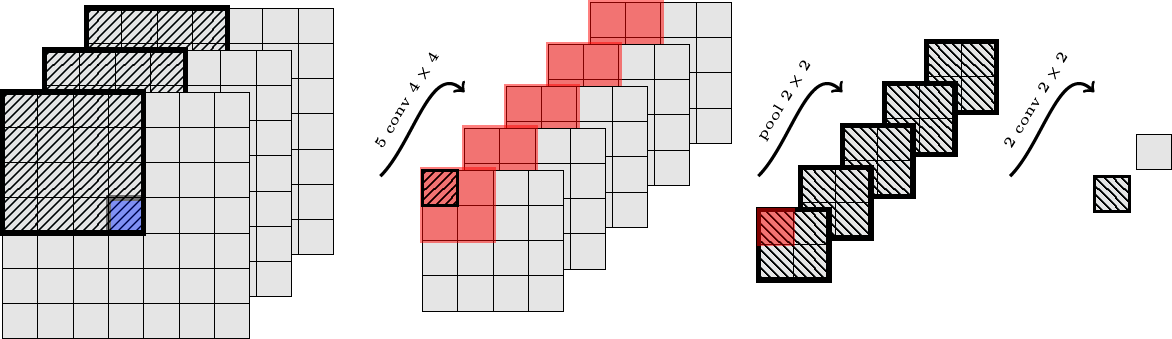
\includegraphics[scale=0.19]{mlp-cw3-template/Figures/ConvNet.png}}
% \caption{}
% \label{fig:ConvNet}
% \end{center}
% \vskip -5mm
% \end{figure} 

\subsection{Fully Convolutional Network}

A Fully Convolutional Network (FCN) \cite{Long2015FullyCN} is a type of Convolutional Neural Network (CNN) that was specifically designed for semantic segmentation tasks (see Figure \ref{fig:fcn}), it is built from only locally connected layers such as convolutional, max pooling and up-sampling layers. Therefore, a FCN does not use fully-connected layers or multilayer perceptrons. In a CNN, these are usually found at the end of the network to make one classification decision for a whole image. However, for semantic segmentation, we want to make predictions on a per-pixel basis. Therefore, the fact that fully-convolutional layers discard local spatial information in favour of a global predictions, makes them unsuitable in this problem domain.

\begin{figure}[htbp]
\vskip 5mm
\begin{center}
\centerline{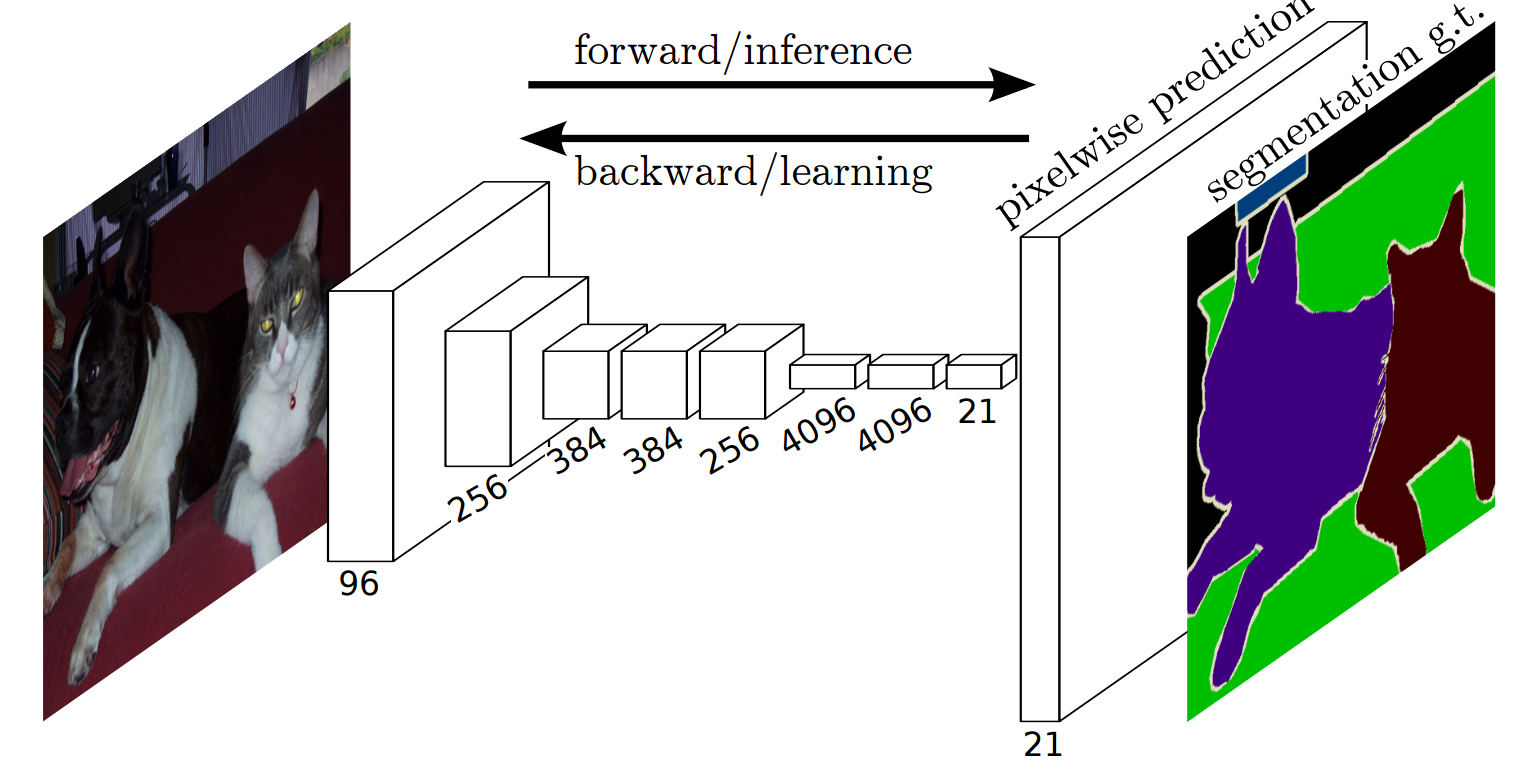
\includegraphics[scale=0.15]{mlp-cw3-template/Figures/fcn.png}}
\caption{Fully convolutional networks can efficiently learn to make dense predictions for per-pixel tasks like semantic segmentation \cite{Long2015FullyCN}.}
\label{fig:fcn}
\end{center}
\vskip -5mm
\end{figure} 

The input and labels are both 3D images, where the dimensions are $C$ x $H$ x $W$. $C$ is the channel dimension and $H$ and $W$ are the spatial dimensions, corresponding to height and width. In the label space, the color channel $C$, is 1 because it is a black and white mask. For the raw microscopic nuclei images, the number of channels $C$ is 3. The output of the segmentation network is a binary mask and so has the same dimensions as in the label space.

To obtain an output, the network must make predictions on a per pixel basis resulting in a segmentation map/mask. The FCN has two paths, an up-sampling path and a down-sampling path. The down-sampling path is used to extract semantic information from the whole picture, while the up-sampling path is used to produce precise localisation of the predictions. In the up-sampling path, we often use skip connections. These skip connections are only used in variants of the original FCN e.g. FCN-8s and FCN-16s. Skip connections allow for the recovery of fine-grained spatial information that is often lost in max pooling/down-sampling. The skip connection bypasses one or more layers, which allows merging/adding of the context (from down-sampling) and the spatial information (from up-sampling).

In our implementation, we used the variant of FCN called FCN-8s, which we trained with VGG-16 network initialisation - removing the fully connected layers from the end of it. VGG-16 was used for the first half of the network (downsampling path) and a custom upsampling path was used based on the FCN-8s implementation discussed in section 4.2 of the original FCN paper \cite{Long2015FullyCN}. Our custom upsampling path consisted of 5 transposed convolutional layers with batch normalisation between them. Each transposed convolutional layer used a filter size of (3, 3) and a stride value of 2. At the end, a 1x1 convolutional layer is used to make the final predictions.

\subsection{U-Net}
We will also explore the U-Net model \cite{Ronneberger2015UNetCN}, which has proved to yield great results in the biomedical image domain. The U-Net model was designed based on the FCN model \cite{Long2015FullyCN} and is also Fully Convolutional itself. The difference in these models is that in the FCN, the whole of the decoder half of the network is used for upsampling (to provide precise localisation of predictions). In the U-Net implementation, the output from the first half of the network (encoder) is concatenated with the upsampled counterpart on the other half of the network. Therefore, in the U-Net implementation, the decoder/second half of the network is in the feature space and the classification is done at the very end. The architecture of a U-Net can be seen in Figure \ref{fig:UNET}, the symmetric nature of this model gives it the ``U'' shape.

A major benefit of U-Net is that is can be trained end-to-end with very few images, while still providing a very high performance compared with other methods such as FCN and Mask-RCNN. Given that our Kaggle dataset is limited and only has around 660 total images before data augmentation, the U-Net model should be a very appropriate model.

\begin{figure}[htbp]
\vskip 5mm
\begin{center}
\centerline{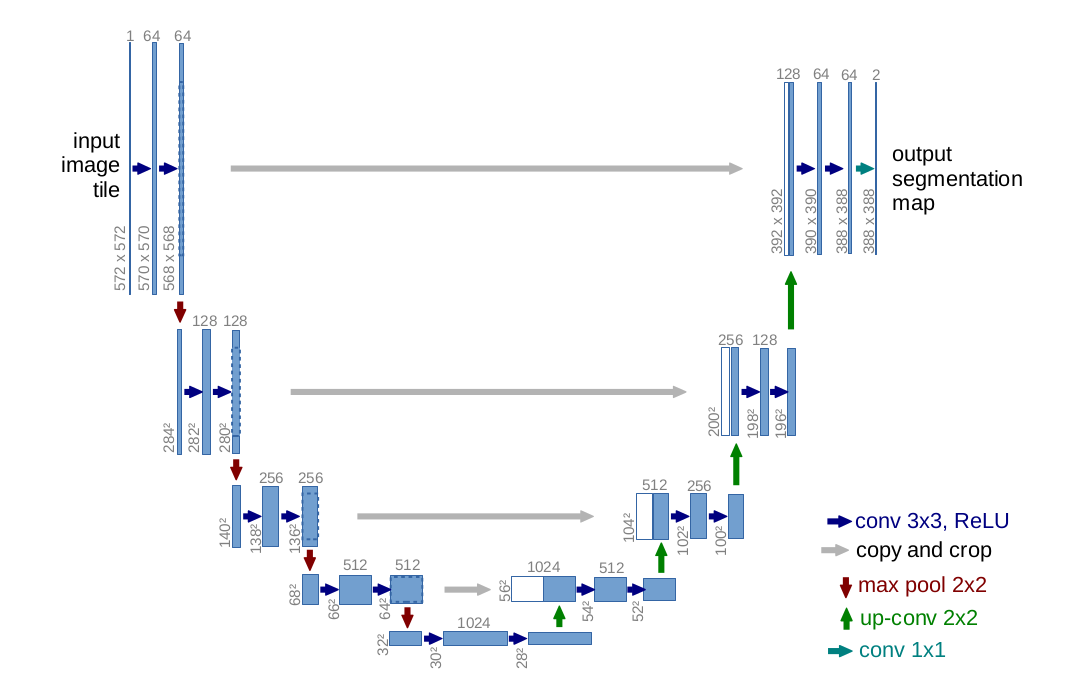
\includegraphics[scale=0.25]{mlp-cw3-template/Figures/unet.png}}
\caption{Illustration of U-Net architecture \cite{Ronneberger2015UNetCN}.}
\label{fig:UNET}
\end{center}
\vskip -5mm
\end{figure} 

The architecture that we will use consists of a series of 3x3 convolutional layers with ReLU activation followed by 2x2 max pooling with a stride of 2 (for downsampling). In the upsampling path, this process is reversed and we use deconvolutions/transposed convolutions in the other direction. At the end, a 1x1 convolution is used to produce a segmentation map and a class for each pixel.

\subsection{Image Preprocessing}
\label{sec:ImgPreProcess}

In an attempt to combat our small dataset and to compare how U-Net and FCN improve with a larger dataset we decided to preprocess the available images to expand our dataset. We used certain techniques outlined in \cite{DataAugmentation} in the following order:
\begin{enumerate}
    \item Flip the image randomly.
    \item Rotate the image a random angle.
    \item Scale the image a random amount.
    \item Translate the image a random distance.
\end{enumerate}
We did this random image manipulation to each image 3 times, increasing our training set from 500 images to 2000 - the original 500 and the three manipulated copies. An example of the image augmentation workflow can be seen in Figure \ref{fig:ImgAugWorkflow}.

\begin{figure}[htbp]
\vskip 5mm
\begin{center}
\centerline{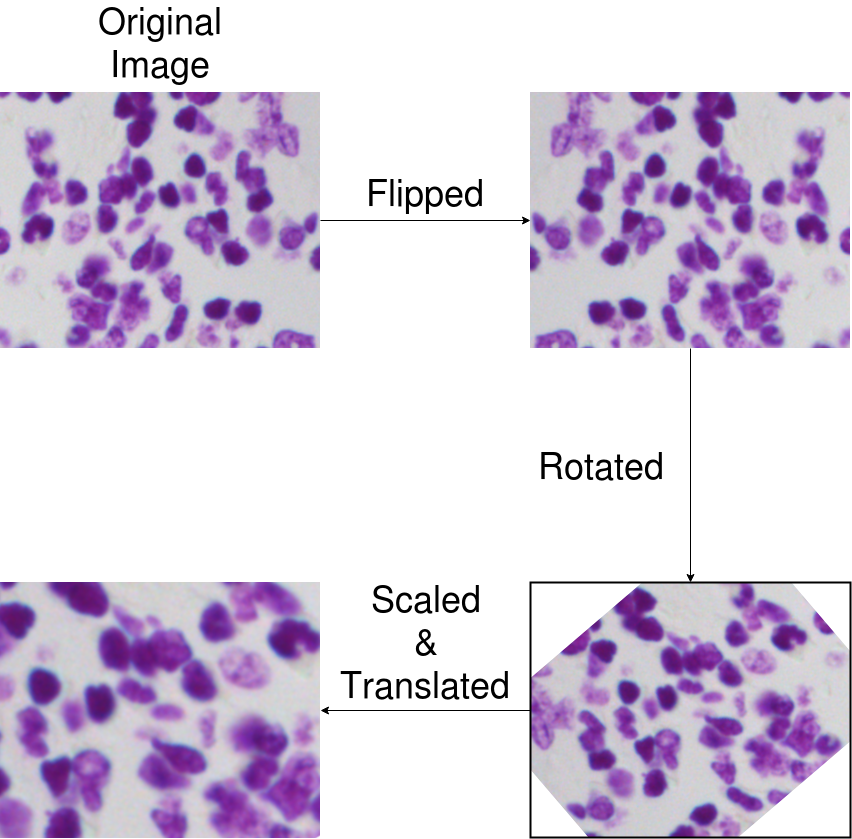
\includegraphics[scale=0.25]{mlp-cw3-template/Figures/AugmentationWorkflow.png}}
\caption{Image Augmentation Workflow}
\label{fig:ImgAugWorkflow}
\end{center}
\vskip -5mm
\end{figure} 

\section{Experiments}
\label{sec:expts}
In the previous section, we mentioned the architectures of the networks that we decided to use in our final experiments. The U-Net model, was based on the original paper \cite{Ronneberger2015UNetCN}, with only a few minor edits to better fit our dataset. In terms of the FCN model, we had to experiment with design of the upsampling path (the downsampling path was taken from VGG-16). We experimented with using transposed convolutions with a stride of 2 vs using no stride in the transposed convolutional layer following simple bilinear interpolation. After numerous experiments, it became clear that using stride produced much better results than interpolation, we therefore used 3x3 transposed convolutions with a stride of 2 in our final architecture.

\begin{figure}[htbp]
\vskip 2mm
\begin{tabular}{ll}
  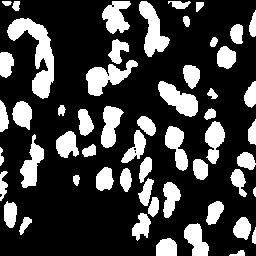
\includegraphics[scale=0.56]{mlp-cw3-template/Figures/ground_truth_nuclei.jpg} &   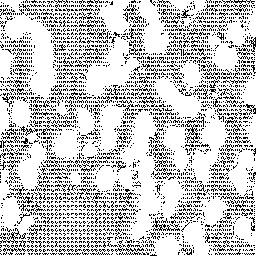
\includegraphics[scale=0.56]{mlp-cw3-template/Figures/fuzzy_prediction.jpg} \\
(a) Ground Truth Mask & (b) Prediction at 3 epochs\\[6pt]
IoU: 1.00 & IoU: 0.413 \\[6pt]
 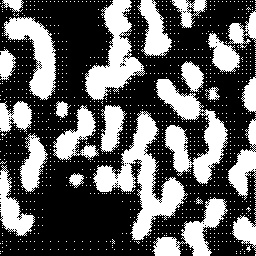
\includegraphics[scale=0.56]{mlp-cw3-template/Figures/predicted_nuclei.jpg} &   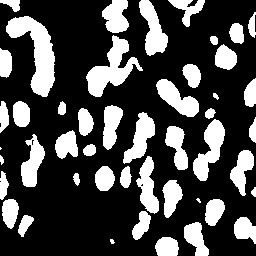
\includegraphics[scale=0.56]{mlp-cw3-template/Figures/great_prediction.jpg} \\
(c) Prediction at 15 epochs & (d) Prediction at 49 epochs\\[6pt]
IoU: 0.632 & IoU: 0.756 \\[6pt]
\end{tabular}
\caption{An example of a ground truth segmentation mask and U-Net's predictions of the mask at various epochs.}
\label{fig:prediction}
\end{figure}

While experimenting with both the FCN and U-Net, we tuned a variety of hyperparameters so that we could compare the models after they had been systematically optimised, not just comparing them at their default values:
\begin{itemize}
    \item Learning Rate
    \item Batch Size
    \item Adam vs RMSProp Optimiser
    \item Momentum and Weight Decay for RMSProp
    \item StepLR Scheduler vs No Scheduler
    \item Lovasz Loss vs Cross-Entropy Loss
\end{itemize}

We ran 4 batches of experiments each with their own grid search, that will be described below. These 4 batches consisted of experiments covering our research questions. Therefore, we included FCN without data augmentation, FCN with data augmentation, U-Net without data augmentation and finally, U-Net with data augmentation. We chose these batches as they would allow us to get comprehensive results to either prove or disprove our hypotheses. 

From our initial experiments, we found that a learning rate of around 0.0001 provided us the best results for both models. After realising this, we decided to vary the learning rate around that value. We used the following values in our hyperparameter search: [0.01, 0.001, 0.0001, 0.00001]. For batch size, we started with a small number of 4 because our dataset is fairly limited in size. However, after a few more experiments we realised that a higher batch size was actually producing better results. Given this, we varied our batch size in the range [8, 16, 32] for our final experiments. 

We also carried out each experiment with both the Adam \cite{Kingma2014AdamAM} optimiser as well as RMSProp. For the Adam optimiser, we used the standard values for beta 1 and beta 2, as specified in the original Adam paper. These values are 0.9 and 0.999 respectively, and we decided not to change these as it would lead to our grid search being too large. We varied the hyperparameters of RMSProp by changing the momentum and weight decay. We changed the momentum a small bit from the default value, 0.9, to try and achieve slight performance increases with the optimiser. We used momentum values of [0.88, 0.90, 0.92], in our experiments. For weight decay, we tried two values that are commonly used in FCN and U-Net models and can be found in many implementations online. These weight decay values are [0.00005, 0.0001]. Finally, we ran all of our experiments using a StepLR scheduler and without using a scheduler. After some initial results, changing both gamma and step size, we decided to use the default values of 0.1 for gamma and a step size of 30.

Initially, we ran our experiments using Cross-Entropy loss as this is a standard and very successful loss function used in many semantic segmentation tasks. However, we found a custom loss function called Lovasz loss \cite{berman2018lovasz}, that was designed to directly optimise the IoU metric and so we believed this would be a very interesting metric to analyse. After initial experiments and a small amount of tuning, we found that the metric worked well producing some satisfactory IoU scores. Given this, we decided to add it into our experiments. We ran every experiment with both Cross-Entropy loss and Lovasz Loss. We then compared the time/accuracy differences of both models, using the two different loss functions. In Table \ref{tab:loss_functions}, we have summarised the results of our experiments into the two loss functions. As we can see, the Lovasz loss function seems to produce worse results than the Cross-Entropy loss function for U-Nets. However, for FCNs the Lovasz loss function was better. We therefore recommend the use of the standard Cross-Entropy loss function for U-Nets and the Lovasz loss function for FCNs. Also, it is clear that training using U-Net offers speed advantages over FCN training. When using a larger dataset, more epochs and carrying out a grid search - the differences in time between these models become more pronounced. U-Net offers not just accuracy boosts but also efficiency boosts. To see examples of training progression on the dataset, from epoch to epoch, refer to Figure \ref{fig:prediction}.

\begin{table}[htbp]
\vskip 3mm
\begin{center}
\begin{small}
\begin{sc}
\begin{tabular}{lcccr}
\hline
\abovespace\belowspace
Loss Function & Time (s) to 50 epochs & Accuracy \\
\hline
\abovespace
All pixels are nuclei & 0 & 0.1318 \\
\\
FCN w/ Lovasz & 4982 & 0.7546 \\
FCN w/ Cross-Entropy & 4971 & 0.7369 \\
\\
U-Net w/ Lovasz & 4610 & 0.7694 \\
\belowspace
U-Net w/ Cross-Entropy & 4588 & 0.7897\\
\hline
\end{tabular}
\end{sc}
\end{small}
\caption{The average accuracy and time to 50 epochs (on validation set) for FCN and U-Net with both Lovasz-Loss and Cross-Entropy loss, over 10 controlled experiments and default parameters.}
\label{tab:loss_functions}
\end{center}
\vskip -3mm
\end{table}

As mentioned above, we ran 4 batches of experiments. Firstly, we ran the 2 batches without data augmentation and analysed the results. From these results, we extracted the model parameters of the best 10 models from both grid searches. These 10 models, for both FCN and U-Net, were then retrained with our data augmentation workflow integrated into the processing pipeline. We decided to use the top 10 models as we wanted to evaluate the boosts that data augmentation gave to the very best models, no to weak models that we wouldn't use in practice. An average IoU was then calculated over the 10 models (on the validation set) and the effect of adding data augmentation can be visualised in Figure \ref{fig:augmentationbarchart}. As we can see from this visualisation, the average IoU increases by 0.559\% when data augmentation is added to FCN and 1.229\% when it is added to U-Net. This shows that, even though U-Net works better with smaller data, it still benefits more from the data augmentation than FCN does. 

\begin{figure}[htbp]
\vskip 5mm
\begin{center}
\centerline{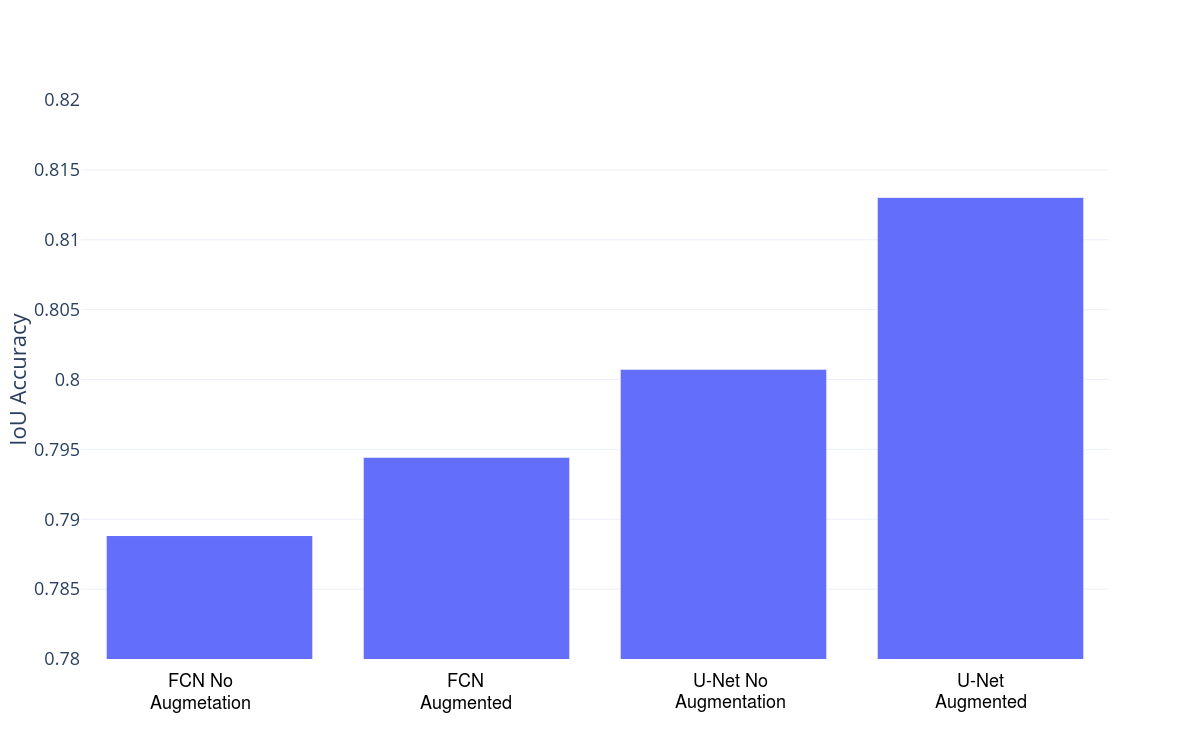
\includegraphics[scale=0.20]{mlp-cw3-template/Figures/BarChart.png}}
\caption{The effect of data augmentation on the IoU accuracy of FCN and U-Net models.}
\label{fig:augmentationbarchart}
\end{center}
\vskip -5mm
\end{figure}

After this, we took the 3 models with the highest validation accuracy for both FCN and U-Net - using data augmentation, and applied them to the held out test set, so we could get results on unseen data which would potentially highlight any signs of overfitting. The results on the test set from these models can be seen in Table \ref{tab:best_models}. As we can see, U-Net performed slightly better than FCN, as we expected. Given that it is also faster to train (see Table \ref{tab:loss_functions}), we recommend using U-Net for semantic segmentation in biomedical applications. We believe it performed better because, it is a lot more lightweight and can deal with our small data problem a lot better than FCN can. Also, the added complexity in U-Net of concatenating the encoder part of the network to the decoding part, seems to have added a sharpness around the edge of the predictions, adding some space between nuclei that were previously merged.

\begin{table}[htbp]
\vskip 3mm
\begin{center}
\begin{small}
\begin{sc}
\begin{tabular}{lcccr}
\hline
\abovespace\belowspace
Model & Test Accuracy \\
\hline
\abovespace
FCN 1 & \textbf{0.7896} \\ 
FCN 2 & 0.7894 \\
FCN 3 & 0.7878 \\
\\
U-Net 1 & 0.8051 \\
U-Net 2 & \textbf{0.8089} \\
\belowspace
U-Net 3 & 0.8039\\
\hline
\end{tabular}
\end{sc}
\end{small}
\caption{The accuracy on the test set of the top 3 best models on the validation set, for both U-Net and FCN.}
\label{tab:best_models}
\end{center}
\vskip -3mm
\end{table}

Out of the top 3 models for both U-Net and FCN the batch size was 32 in every case. This went against our earlier intuition, we expected a smaller batch size to work better because of the small dataset. However, 32 seems to be the optimal value - after a few experiments with 64 we didn't notice any further improvements. In terms of learning rate, we didn't find that any of the learning rates produced significantly better results than the others. In the top 10 models for both U-Net and FCN, we found that every learning rate that we investigated, was used in one of our best models. This is likely due to the fact that other hyperparameters had a larger effect on the final results.

For U-Net and FCN we found that the RMSProp optimiser was found in 9/10 of our highest scoring models and all of the top 3 models. We recommend using the RMSProp algorithm, however, we believe Adam's poor performance  may be due to insufficient tuning of the beta (beta 1 and beta 2) values in the optimiser's parameters - an oversight on our part. Only 1/20 of the top models across U-Net and FCN made use of the StepLR scheduler that we included, this was used in an FCN model with 0.7883 accuracy on the validation set. This shows that the inclusion of a scheduler does not help in every case and initial experiments should be done to analyse whether a model would benefit from a scheduler or not. On the other hand, if we had more resources to do a larger grid search we would have liked to have tried using the Cosine Annealing scheduler and perhaps we would have tried changing the step size and gamma values for the StepLR scheduler. The cosine annealing scheduler has worked well for us in the past, in a different report, and may have introduced further accuracy boosts. 

As we mentioned above, the FCN model benefited from the Lovasz loss function with all of the top 3 models using it and 7/10 of the top models. For the top 10 U-Net models, 10/10 of them used the Cross-Entropy loss function. We can see that the Lovasz loss function seems to struggle when used with the U-Net implementation but is very good when integrated into our FCN model. This is interesting because of how closely related the two models are in their architecture. 

The hyperparameters for our best FCN model (FCN 1), see Table \ref{tab:best_models}, are: a learning rate of 0.0001, a batch size of 32, the RMSProp optimiser with 0.88 momentum and weight decay of 0.00005, Lovasz loss function and does not use any sort of scheduler. On the other hand, the hyperparameters for our best U-Net model (U-Net 2), see Table \ref{tab:best_models}, are: a learning rate of 0.00001, a batch size of 32, the RMSProp optimiser with 0.9 momentum and 0.00005 weight decay, Cross-Entropy loss function and does not use a scheduler. 

In Figure \ref{fig:learninggraphs}, the learning curves can be seen for these two best models, on the validation set - both the loss and IoU accuracy are plotted against the epoch training progression. Note, the loss functions are different for both models, as described above.

\begin{figure}[htbp]
    \vskip 5mm
    \centering
    \subfloat[IoU vs Epoch]{{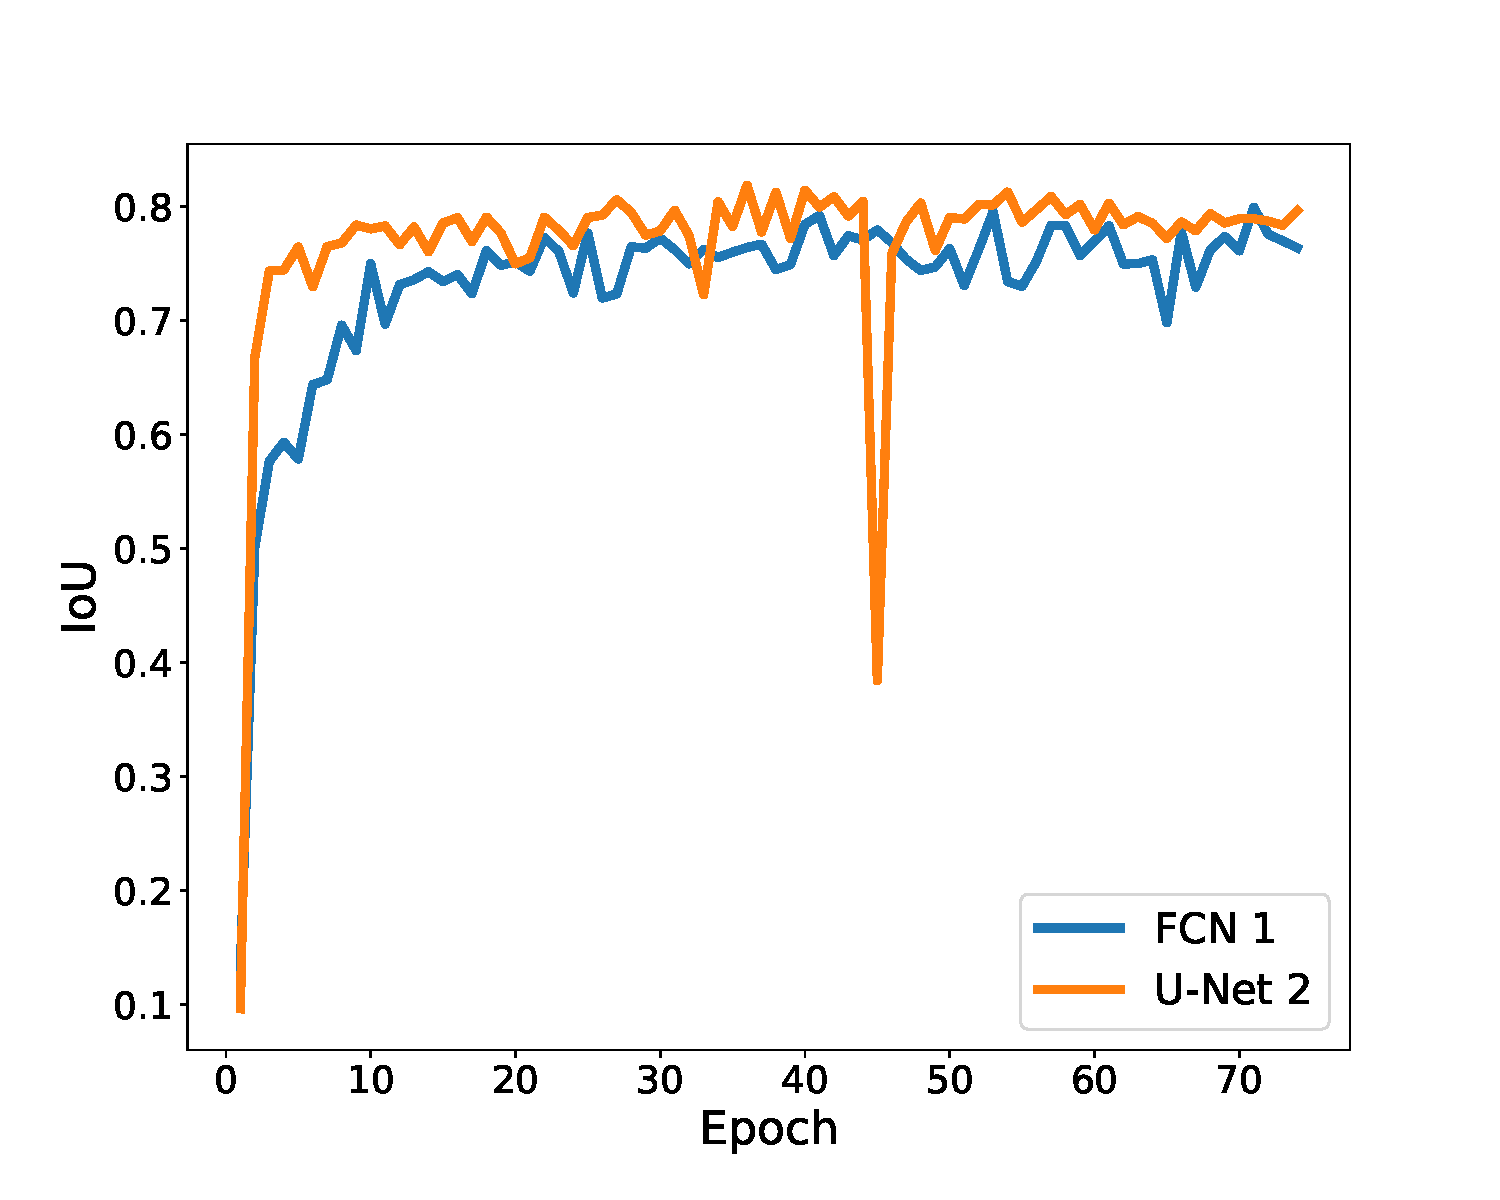
\includegraphics[scale=0.3]{mlp-cw3-template/Figures/IoUVsEpoch.pdf}}}%
    \qquad
    \subfloat[Loss vs Epoch]{{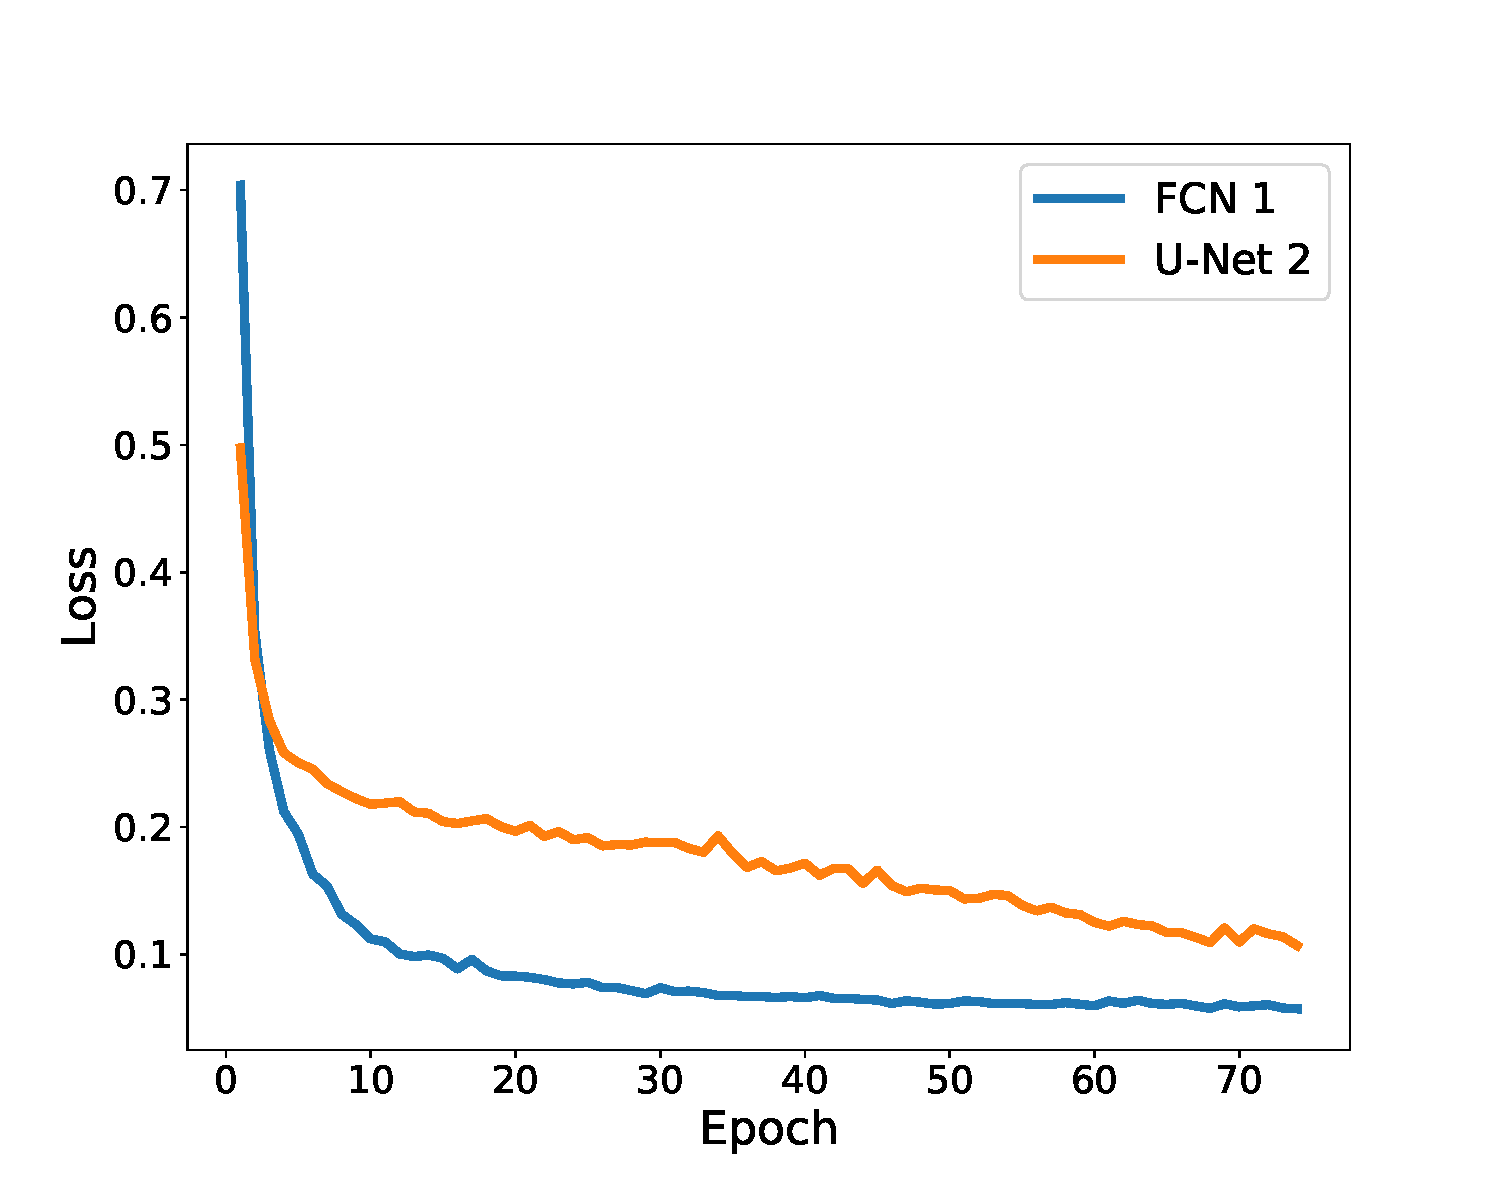
\includegraphics[scale=0.3]{mlp-cw3-template/Figures/LossVsEpoch.pdf} }}%
    \caption{Learning graphs for the best FCN and U-Net model on the validation set, the best models can be seen in Table \ref{tab:best_models}.}%
    \label{fig:learninggraphs}%
    \vskip -5mm
\end{figure}

\section{Conclusion}
\label{sec:concl}
\textbf{Why was U-Net more accurate?}

We believe the reason for the U-Net accuracy boosts is its use of concatenation in the upsampling stage, which allows the U-Net to bring back information that is lost in the downsampling stage via pooling layers and stride. Including the data from the downsampling stage into the upsampling stage allows for higher resolution representations to be included in the feature space. Having these representations of the original image, in the feature space, allows for better localisation - which should further prevent/reduce the amount of merging nuclei. In our opinion, this is the reason why U-Net performs slighly better overall than FCN - FCN loses some of this important localisation, in the downsampling stage. 

\textbf{Why was U-Net slightly faster than FCN?}

In the results of our run time checks (seen in Table \ref{tab:loss_functions}), we found that U-Net was somewhat faster than FCN. Our FCN model included a pre-trained VGG model at the encoder stage which should have offered significant speed ups. However, the U-Net model which trained end-to-end actually trained faster. In addition to this, they both used 5 layers of upsampling in their respective decoder phases, most of the training time likely came from our data augmentation workflow. We believe the high utilisation of U-Net and its ability to learn from very small amounts of data make it an impressive model.

\textbf{Why did data augmentation boosts IoU accuracy results?}

We found that data augmentation was important in our experiment and if we had more time, we would have liked to have implemented a grid search over a combination of various workflows, including the techniques we mentioned e.g. random cropping, rotation etc. We would have then been able to optimise our workflow and find even greater boosts to the network. However, we believe that our workflow was still very good after and showed the best accuracy improvements in our initial tests and throughout our implementation. Our experiments showed the importance of data augmenatation for both models, as we can see in Figure \ref{fig:augmentationbarchart}. In our opinion, the reason for this is simply the added amount of data that is available to our models, around 1500 more training examples - this additional relevant data helped reduce any overfitting in our system that was caused by our limited dataset. These distortions of the original image that we added allow our networks to differentiate between noise in the data and relevant features/signals.

\subsection{Related Work and Future Improvements}

% Related Work:

% - Talk about Kaggle approaches.
% The best kaggle solution used Mask RCNN

% - Find new papers 2018/2019 that do a similar task (biomedical segmentation) and talk about their approach.

% - Future work - Mask RCNN and why we think this might be a good approach vs what we attempted.

In recent years, there have been a variety of attempts at semantic segmentation in this domain because of its importance for researchers and the benefits it has already yielded. In \cite{comparitivestudy} they compared fairly simple models; Otsu's method, k-means clustering, mean shift, Chan–Vese method, and graph cut method to compare how they perform at cell segmentation. These models seemed to perform well without requiring the complexity that was present in our models. The training time of these models is faster than ours due to their simplicity but we believe that our models would outperform theirs especially with this limited dataset.

There has also been research into unsupervised cell segmentation \cite{unsupervisedsegmentation} which claims to achieve 99.47\% segmentation rate. We didn't have time to see how their model performs on our dataset, and calculate its IoU accuracy, but we believe this could be interesting future work.

Mask RCNN seemed to be one of the highest performing models on the Kaggle competition as was used by \cite{kaggle11thplace}. But as mentioned in section \ref{sec:intro} this solution and other Mask RCNN models used other datasets to improve their performance. 
Nevertheless for future work and improvements, we could approach Mask RCNN \cite{MaskRCNN}, after acquiring more data and compare it with our existing models. We believe this is an interesting comparison because Mask RCNN's approach of instance segmentation should allow for better separation of nuclei. The instance segmentation map could then be converted into a semantic segmentation map, potentially producing gains on U-Net. We believe there would be drawbacks to Mask RCNN, because it is much slower as it requires a two-phase training approach; it must optimise for an RPN (Region Proposal Network), then predict boundaries and masks for all the nuclei.

Also, we are very interested in investigating the importance of post-processing, given that we have extensively covered pre-processing. Using a variety of techniques such as Conditional Random Fields would allow us to `clean' up the image, this has worked well in similar semantic segmentation tasks \cite{Shrestha2018ImprovedFC}. By including this technique to sharpen around the image, a lot of accuracy would be gained between nuclei and boundary areas surrounding the nuclei. Currently, we are predicting an area, around the nuclei, that is slightly bigger than it should be.


\bibliography{example-refs}

\end{document} 

